% !TEX encoding = UTF-8 Unicode
%%%%%%%%%%%%%%%%%%%%%%%%%%%%%%%%%%%%%%%%%%%%%%%%%%%%%%%%%%%%%%%%%%%%%%%%%%%%%%%%%%%%%%%%%%%%%%%%%%%%%%%%%
%%
%%  Migrated from ASME Conference (asmeconf) format to ASME Journal (asmejour) format.
%%  Content unchanged — only formatting adapted.
%%
%%%%%%%%%%%%%%%%%%%%%%%%%%%%%%%%%%%%%%%%%%%%%%%%%%%%%%%%%%%%%%%%%%%%%%%%%%%%%%%%%%%%%%%%%%%%%%%%%%%%%%%%%

\documentclass[subscriptcorrection,upint,varvw,balance,hyphenate]{asmejour}

%%%%%  pdf metadata  %%%%%%%%%%%%%%%%%%%%%%%%%%%%%%%%%%%%%%%%%%%%%%%%%%%%%%%%%%%%%%%%%%%%%%%%%%%%%%%%%%

\hypersetup{%
	pdfauthor={Reihane Arabpoor, Lucas Chen, Azadeh Haghighi},
	pdftitle={Toward Reliable Hybrid Electronics: Understanding the Role of Surface Roughness in Aerosol Jet Printing},
	pdfkeywords={Aerosol jet printing, Hybrid electronics, Printed electronics, Additive manufacturing surface roughness},
	pdfsubject = {Effect of surface roughness on aerosol jet printing for hybrid electronics},
}

%%%%  Journal name %%%%%%%%%%%%%%

\JourName{JMNSE}

%%%%%%%%%%%%%%%%%%%%%%%%%%%%%%%%%%%%%%%%%%%%%%%%%%%%%%%%%%%%%%%%%%%%%%%%%%%%%%%%%%%%%%%%%%%%%%%%%%%%%%%

\allowdisplaybreaks

\usepackage{hologo}
\usepackage{subcaption}
\usepackage{float}
\usepackage{xspace}
\newcommand{\rev}[1]{\textcolor{black}{#1\xspace}}
\newcommand{\savesectionspace}{\vspace{-1mm}}


\begin{document}

\SetAuthorBlock{Reihane Arabpoor}{%
Department of Mechanical and Industrial Engineering,\\
University of Illinois Chicago,\\
Chicago, IL, USA\\
}
\SetAuthorBlock{Lucas Chen}{%
Department of Mechanical and Industrial Engineering,\\
University of Illinois Chicago,\\
Chicago, IL, USA
}
\SetAuthorBlock{Azadeh Haghighi\CorrespondingAuthor}{%
Department of Mechanical and Industrial Engineering,\\
University of Illinois Chicago,\\
Chicago, IL, USA\\
email: ahaghi3@uic.edu
}


\title{Toward Reliable Hybrid Electronics: Understanding the Role of Surface Roughness in Aerosol Jet Printing}

\keywords{Aerosol jet printing, Hybrid electronics, Printed electronics, Additive manufacturing surface roughness}

%%%%%  ABSTRACT  %%%%%%%%%%%%%%%%%%%%%%%%%%%%%%%%%%%%%%%%%%%%%%%%%%%
%%
%% Abstract should be 200 words or less
\begin{abstract}
Recent advancements in hybrid additive manufacturing (AM) of electronics have enabled the fabrication of compact, high-quality, and high-resolution three-dimensional electronic systems. However, these developments raise new challenges in process planning and optimization to ensure reliable performance of the final part. Among the various techniques available for printed electronics, aerosol jet printing (AJP) stands out for its versatility and compatibility with hybrid AM systems. Its ability to deposit materials in a contactless manner with up to five axes of motion allows the printing of conductive traces, embedded sensors, and interconnects on complex or nonplanar surfaces with high aspect ratios. Furthermore, AJP's compatibility with both conductive metallic inks and non-conductive polymer materials enables the integration of functional and insulating layers, thereby enhancing the durability and multifunctionality of printed electronic components.
Despite these advantages, several challenges must be addressed to achieve consistent and high-quality printed features. AJP typically produces line widths and thicknesses on the order of a few microns, while many AM-produced substrates exhibit surface roughness values of similar or even larger magnitude. Such surface variations can disrupt trace continuity and compromise electrical connectivity. Therefore, a comprehensive understanding of how substrate surface roughness influences AJP deposition behavior is critical for effective process and path planning.
This study presents experimental investigations into the effects of substrate roughness on aerosol particle deposition and printed line morphology. The results reveal that surface roughness significantly affects line uniformity and continuity. Additionally, the motion and redistribution of the ink on rough surfaces were found to strongly influence the final quality of the printed traces.
These findings highlight the necessity of integrating surface roughness characterization into the process planning stage for AJP-based hybrid AM. By establishing a foundational understanding of the interaction between surface topography and ink deposition, this work opens new pathways for improving the reliability and precision of embedded and hybrid-printed electronics.

\end{abstract}

\maketitle

\savesectionspace
\section{Introduction}
With recent advancements in additive and smart manufacturing technologies, new opportunities have emerged for fabricating components that were previously expensive or even impossible to produce \cite{ngo2018additive}. The concept of compact three-dimensional (3D) electronics, where complex circuits are embedded within 3D geometries rather than confined to flat, two-dimensional (2D) surfaces, has become increasingly feasible due to these technological breakthroughs \cite{goh20213d,li2019hybrid,child2025printegrated}. Embedding electronics within the body of a component, instead of only on its surface, offers distinct advantages in terms of durability, reliability, and safety \cite{maalderink20183d}. In the case of sensors, internal placement can enable higher measurement accuracy and facilitate early-stage detection of physical or chemical changes within a part \cite{dijkshoorn2018embedded,hassan20233d}.


Hybrid additive manufacturing (AM) has emerged as a promising approach to realize these benefits by integrating two or more AM techniques within a single process. This integration allows simultaneous fabrication of structural and functional elements, such as embedded electronics or sensors, in a unified workflow \cite{li2019hybrid}.

Among the various techniques available for printed electronics, Aerosol Jet Printing (AJP) stands out as one of the most suitable candidates for integration into hybrid AM systems due to its versatility and precision \cite{wilkinson2019review}. AJP can accommodate a wide range of ink viscosities, from metal-based conductive inks to polymer-based dielectric materials \cite{secor2018principles,rodriguez2012dielectric}. Using either pneumatic or ultrasonic atomization, the process generates fine aerosolized droplets that are carried by a nitrogen gas stream toward the deposition head. There, a sheath gas, introduced around the carrier flow, aerodynamically focuses the aerosol stream. The resulting focused jet is ejected through a nozzle as small as 100 µm in diameter, typically operating at a stand-off distance of approximately 3 mm from the substrate \cite{secor2018principles,jeong2023optimization,secor2025additive,gohel2025direct}. This configuration allows AJP to deposit materials onto surfaces with varying roughness profiles and geometrical complexities \cite{arabpoor2025experimental}.

Such adaptability makes AJP highly advantageous for hybrid AM \cite{wilkinson2019review,li2019hybrid}, where printed substrates often exhibit significant variations in surface texture and height. Techniques that rely on close contact or limited depth-of-focus typically lose resolution under these conditions. In contrast, AJP can maintain print resolutions down to just a few micrometers when its process parameters are optimized for the given ink properties and print conditions \cite{secor2018principles, jeong2023optimization}.

Although research on AJP for conformal and non-planar surface printing has grown substantially in recent years \cite{rurup2024understanding,jignasu2023conformal,arabpoor2025experimental}, several critical knowledge gaps remain. In particular, while some studies have explored AJP for interconnects or other electronic features within hybrid AM systems \cite{obeidatfine,werum2022aerosol}, the underlying interactions between AJP-deposited materials and the inherent surface characteristics of AM-produced substrates require further investigation.
\begin{figure}[H]
    \centering
    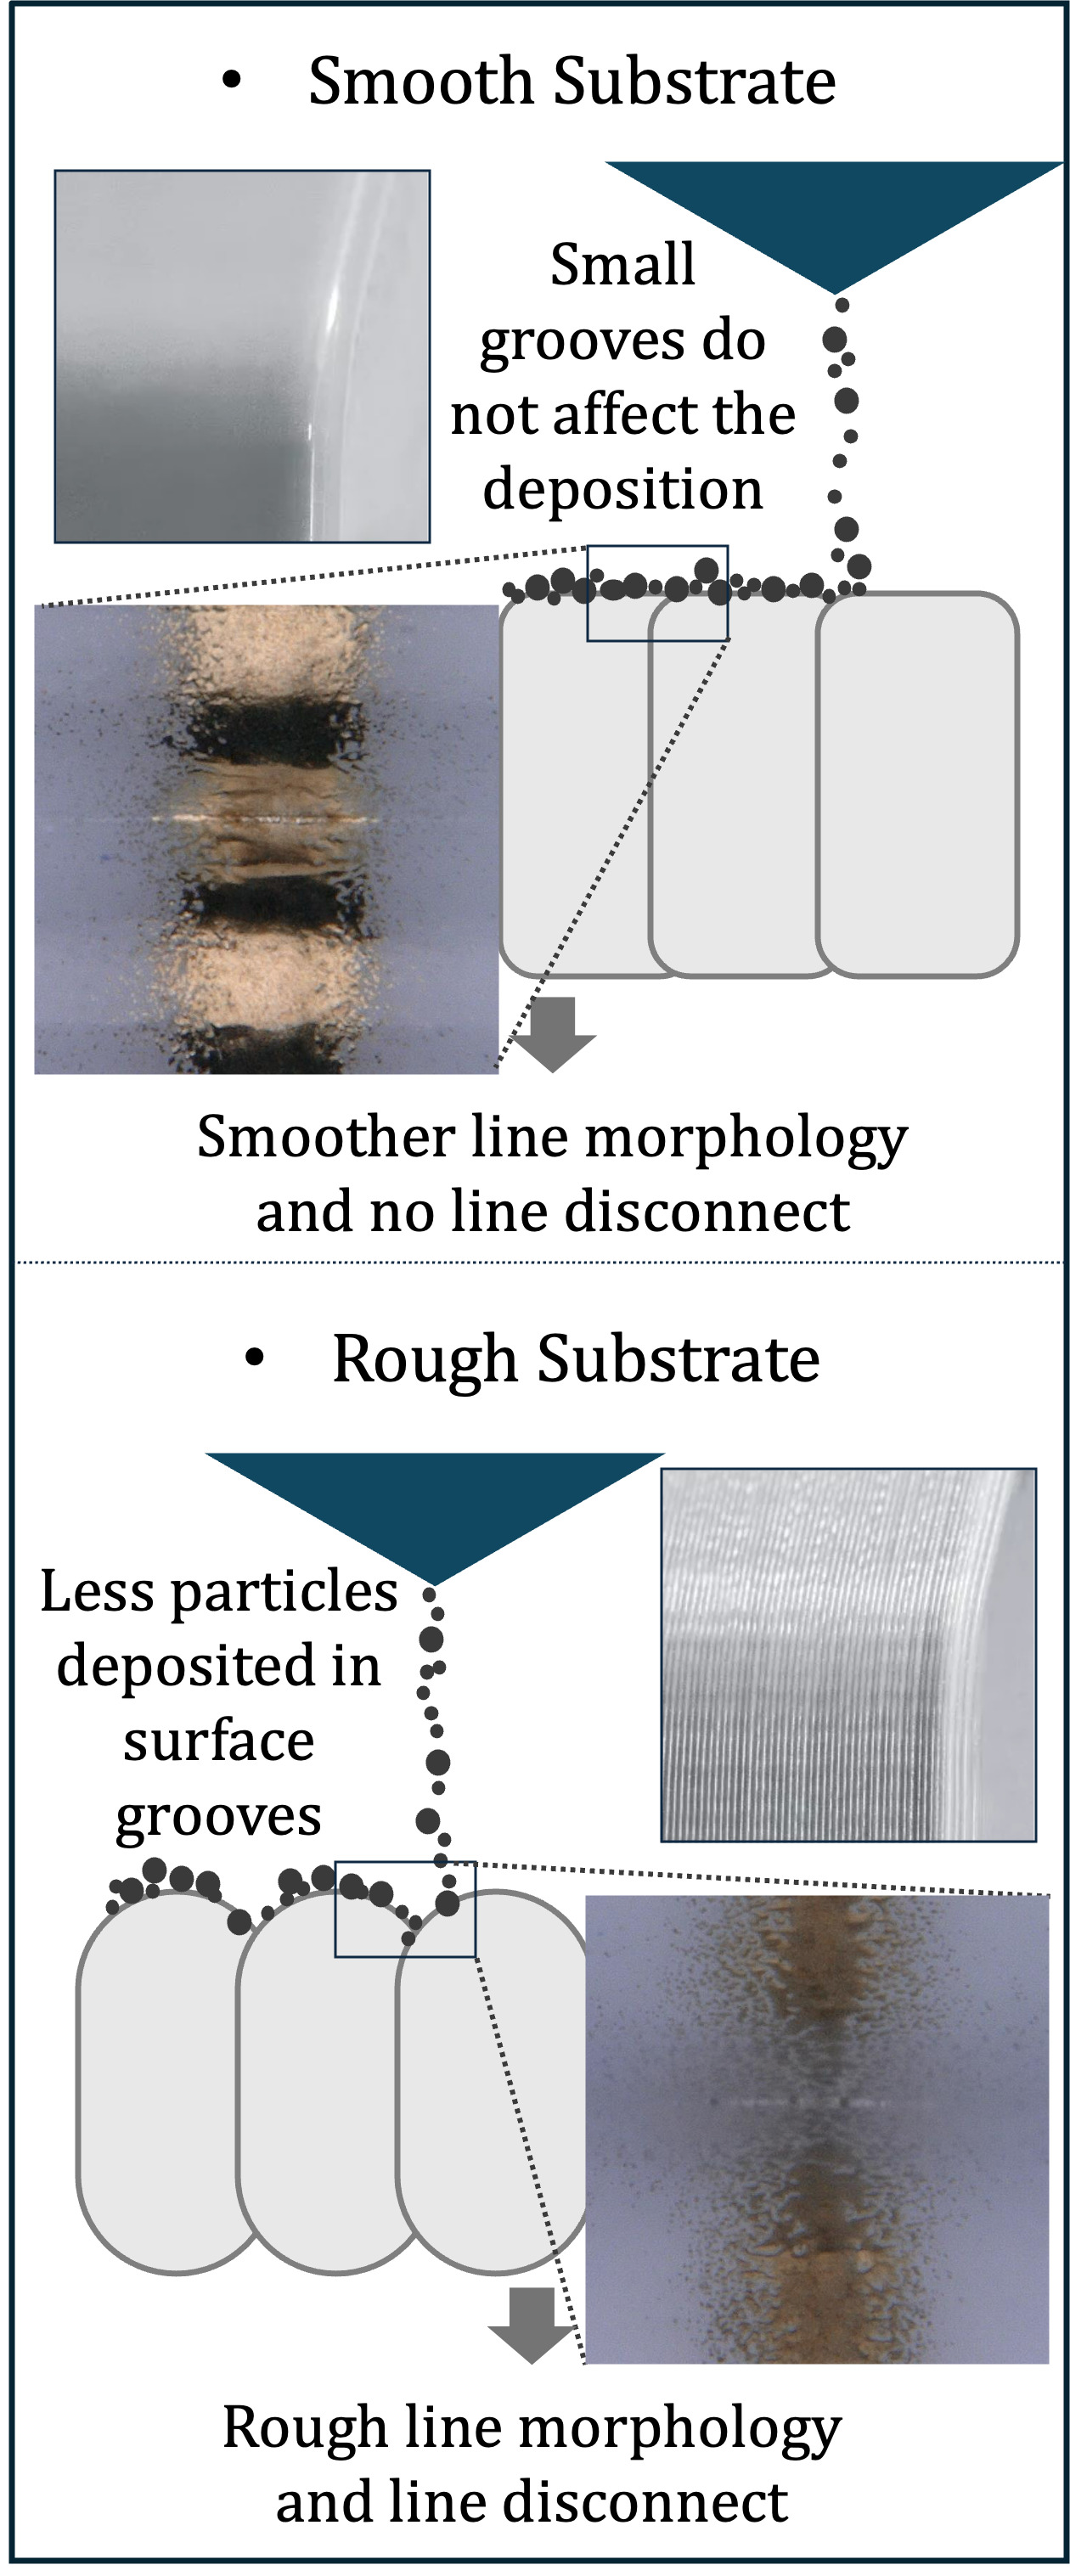
\includegraphics[width=0.9\linewidth]{figs/intro2.jpg}
    \caption{Schematic illustration of the effect of surface roughness on AJP particle deposition. On a smooth surface, the particles form a continuous trace. On a rough surface, deposition in the valleys is incomplete, resulting in partial disconnections and reduced trace continuity.}
    \label{fig:intro}
\end{figure} 



As previously mentioned, one key surface property of AM-fabricated parts is surface roughness \cite{obilanade2021surface}, which often follows a periodic pattern dependent on geometry, process type, and print conditions \cite{ahn2009representation}. This parameter has been extensively characterized in studies focused solely on AM process modeling, with analytical and empirical models capable of predicting surface roughness with high accuracy \cite{wu2019predictive,li2019theoretical}. When AJP is integrated with other AM techniques, it becomes essential to understand how this roughness influences printed line morphology and electrical continuity. Questions arise such as: Can surface grooves cause disconnections \rev{or undesired particle deposition} in printed traces? And if so, how can process planning and parameter optimization mitigate these effects?

In this work, we introduce a systematic approach to evaluate the effect of surface roughness on line connectivity \rev{and variability} of AJP-printed components. To achieve this goal, Fused Deposition Modeling (FDM) substrates were selected as the base material due to the well-established and repeatable surface features characteristic of this process \cite{li2019theoretical}. The FDM samples were fabricated to exhibit a consistent surface pattern while varying the layer height to introduce different roughness depths for experimental comparison. These test cases were then used as substrates for AJP, upon which several conductive traces were deposited under controlled conditions.

Given the high resolution of AJP, which often is smaller than the characteristic size of surface roughness grooves, deposition on such textured surfaces may result in incomplete filling of the grooves. This can cause partial disconnections within the printed traces, where some particles may settle in the valleys but fail to establish full continuity with material deposited in adjacent regions. Figure~\ref{fig:intro} provides a visual illustration of this effect, comparing particle deposition on a smooth surface versus a rough surface. This study systematically investigates this phenomenon through experimental analysis to highlight a critical knowledge gap that warrants further attention from the research community. While the present work focuses on identifying and characterizing this effect, future studies will explore process optimization strategies and potential solutions to mitigate these issues.

%%%%%%%%%%%%%%%%%%%%%%%%%%%%%%%%%%%%%%%%%%%%%%%%%%%%%%%%%%%
% \savesectionspace
% \savesectionspace
\begin{figure}[h]
    \centering
    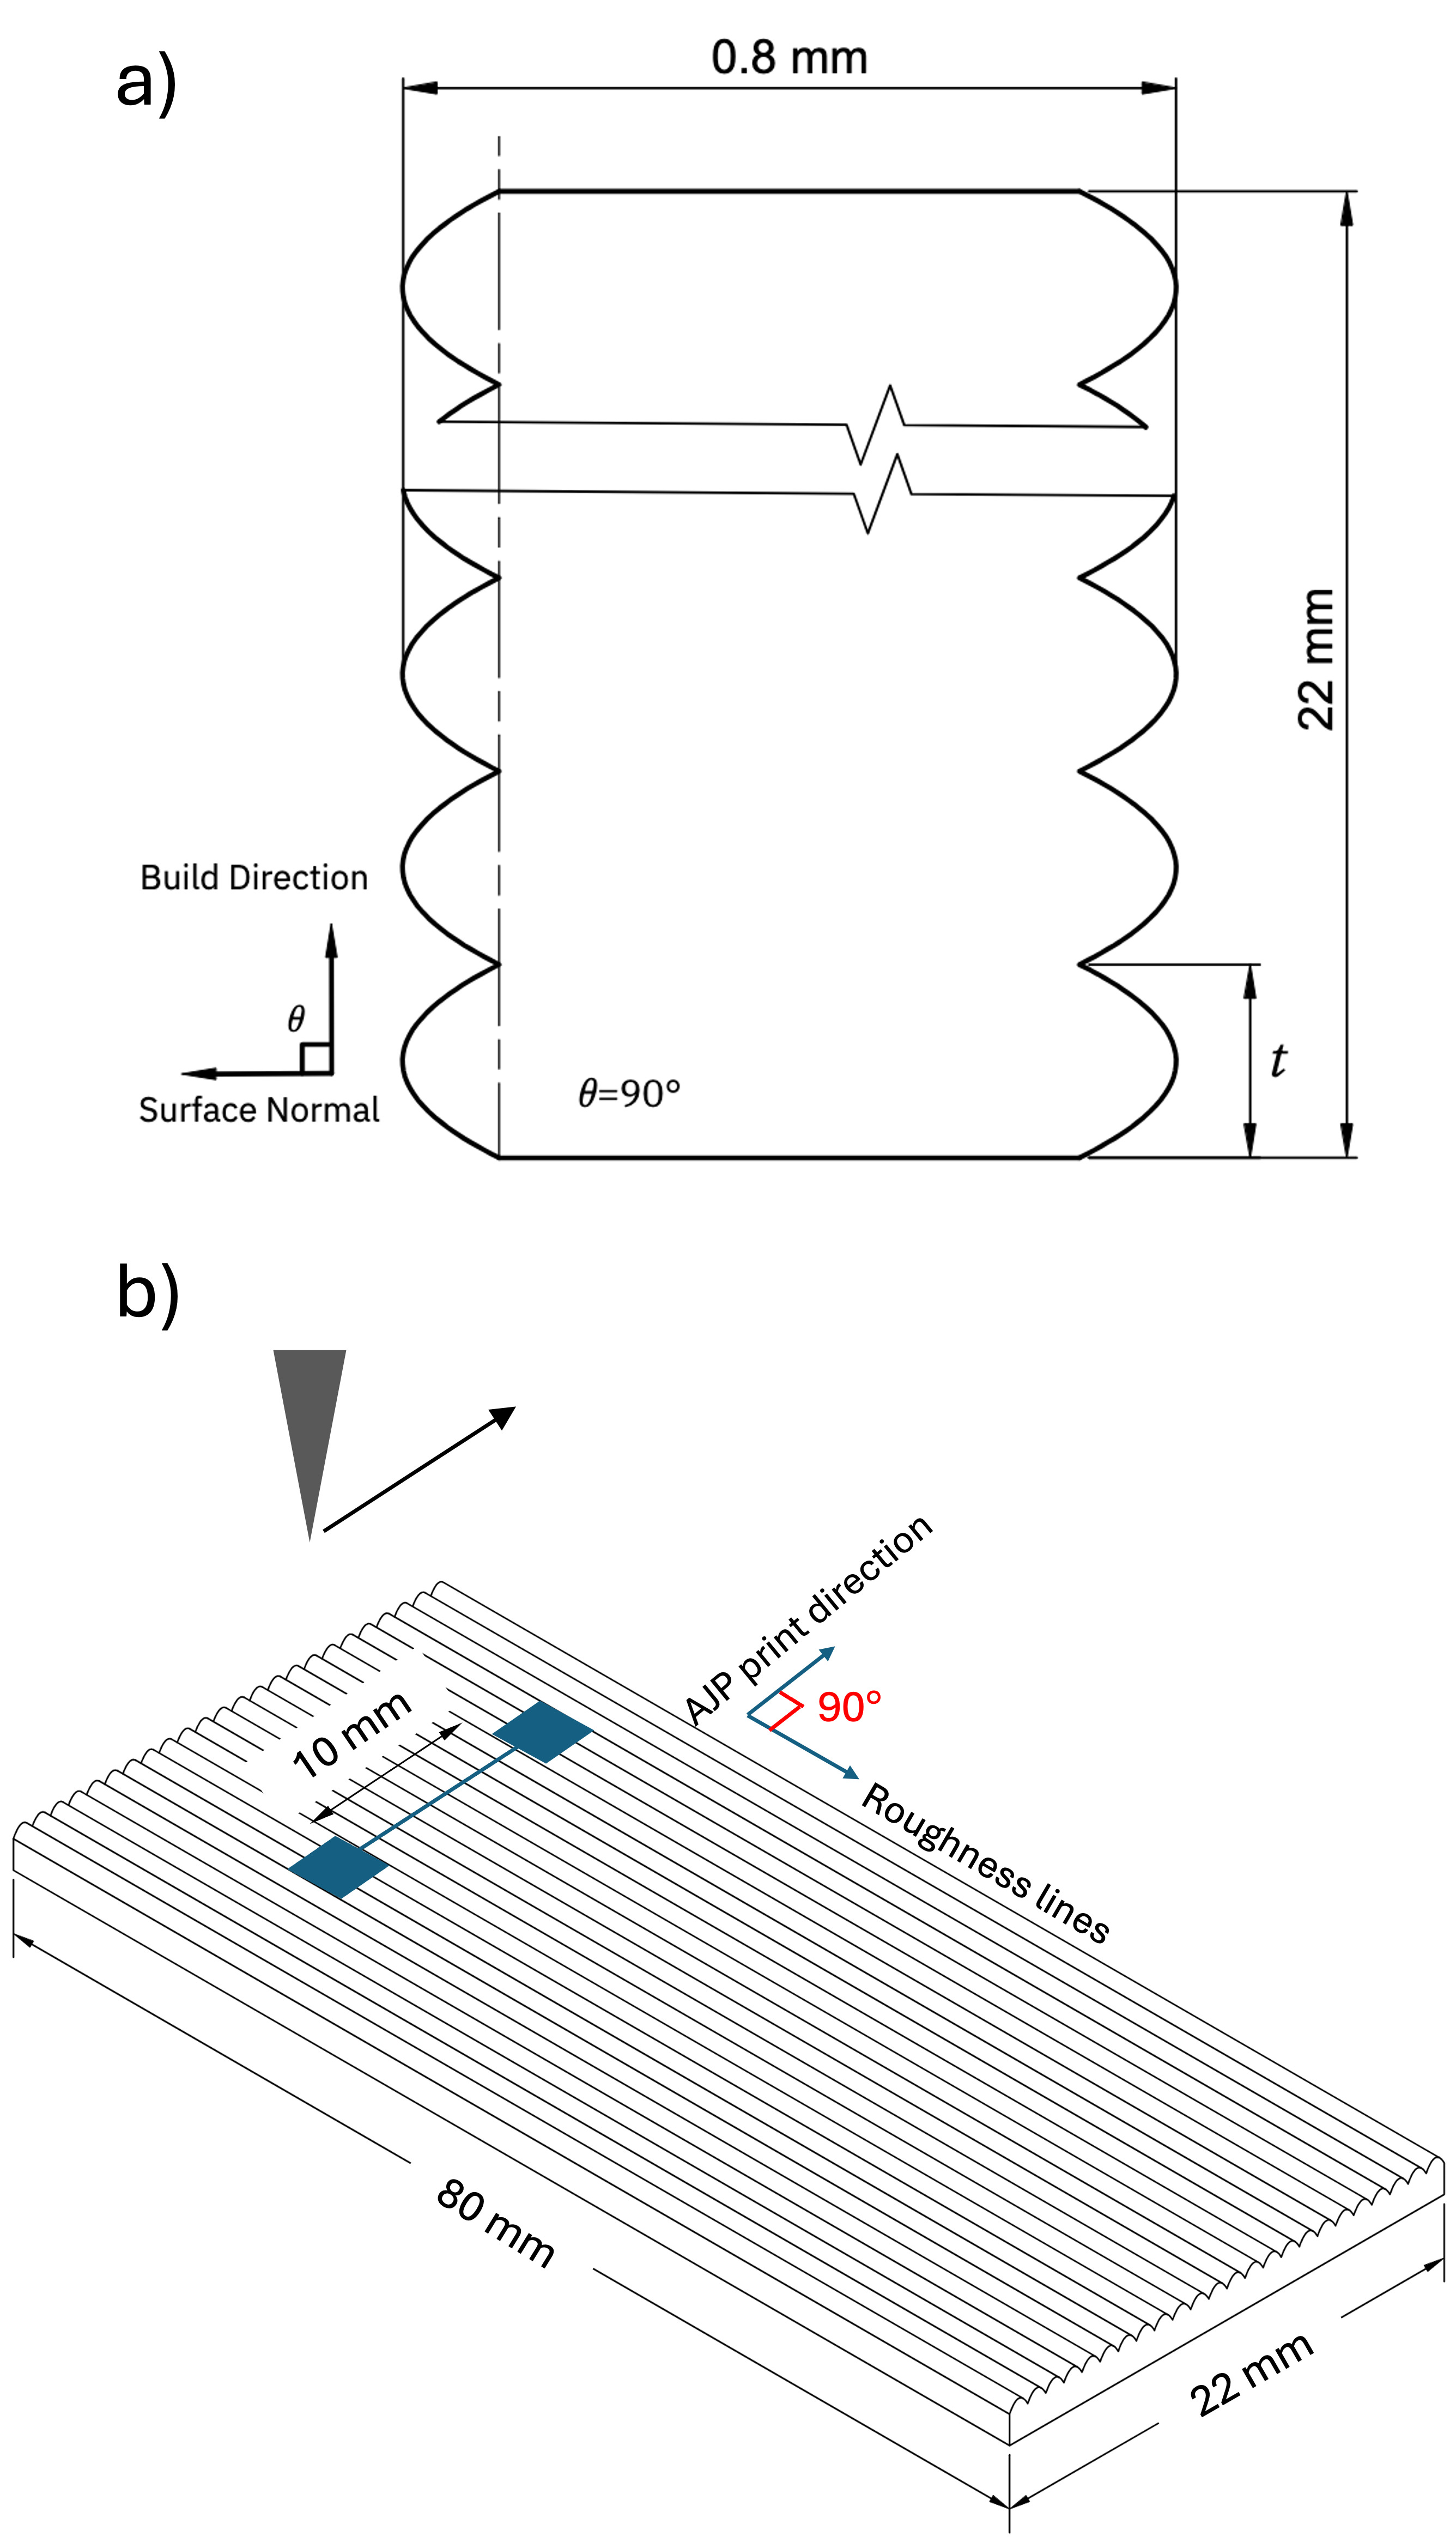
\includegraphics[width=0.98\linewidth]{figs/method2.jpg}
    \caption{Overview of the experimental setup showing (a) the FDM surface roughness profile and (b) the pattern design and print orientation relative to the substrate topography.}
    \savesectionspace
    \label{fig:method}
\end{figure}
% \savesectionspace
% \savesectionspace


\section{Methodology}

In this section, we first provide a brief overview of the theoretical background of the work. This is followed by a detailed description of the experimental procedures for both AJP and FDM, with an emphasis on surface roughness–related parameters. The characterization methods and tests employed in this study are also described.

\subsection{Theory}

Aerosol Jet Printing is fundamentally a multiphase flow process, in which solid particles of the functional material (metal in this study) are encapsulated within a liquid carrier to form aerosol droplets. These droplets are transported by a gas stream and jetted through a nozzle to impact the substrate \cite{secor2018principles,salary2017computational}. The governing physics of AJP on smooth planar surfaces has been extensively studied, providing a thorough understanding of particle dynamics, gas flow, and deposition mechanisms \cite{chen2018effect,salary2017computational,ramesh2023computational}.


When printing on non-smooth surfaces, such as FDM-printed parts with periodic surface roughness, the underlying physics of the process does not change. 

However, the impinging aerosol jet may be affected by the surface topography, leading to modifications in the gas streamlines near the substrate. This is significant because the motion of aerosol particles is influenced by their inertia: particles with low inertia tend to closely follow the gas streamlines. Consequently, any alteration in the local gas flow induced by surface roughness can directly impact particle deposition patterns \cite{rurup2024understanding}.

In this work, we experimentally investigate the effect of surface roughness on AJP deposition. Future studies may extend this work by employing computational fluid dynamics (CFD) simulations to model how surface topography alters the aerosol jet and particle deposition, thereby enhancing the understanding of the underlying physical mechanisms.

\begin{table}[]
\centering % Centers the table on the page
\caption{Summary of AJP process conditions used for parameter variation.} % Added a caption
\label{tab:1} % The label should come AFTER the caption
\begin{tabular}{@{}ccc@{}} % 'l' for labels, 'c' for centered data
\toprule
\textbf{Test}      & \textbf{Stand-off Distance (mm)}                   & \textbf{Print Speed (mm/s)}             \\ \midrule
1    & 3              & 3 \\
2    & 1.5            & 3 \\
3    & 3              & 2 \\
4    & 1.5            & 2 \\ \bottomrule
\end{tabular}
\end{table}


\subsection{Experimental and Characterization Details}
AJP experiments were conducted using an Optomec Aerosol Jet AJ5x system with ultrasonic atomization of Novacentrix silver ink (Metalon JS-A426). 

FDM substrates were fabricated using a FDM printer, similar in design to the Ender3 format , featuring core XZ kinematics for precise control over z-axis movement. The filament utilized was PolyLite PLA Pro, a modified polymer composite consisting of PLA and Polycaprolactone (PCL), a blend formula well known for its enhanced mechanical properties.

Microscopy characterization was conducted using a Keyence VHX-6000 digital microscope. The multi-layer depth composition mode was utilized to capture several focal planes along the z-axis and synthesize them into a single fully focused composite image, enabling clear visualization of the printed line along rough surface profiles.

During AJP, key process parameters, including atomizer gas flow rate (\(8~\mathrm{sccm}\)), sheath gas flow rate (\(50~\mathrm{sccm}\)), and ink temperature (\(25~^{\circ}\mathrm{C}\)), were held constant across \rev{test conditions 1–4}. The standoff distance and print speed were varied to generate four printing conditions, as summarized in Table~\ref{tab:1}. \rev{To investigate the influence of higher deposition rates as a potential mitigation strategy, an additional case study was introduced using an atomizer gas flow rate of \(20~\mathrm{sccm}\) and sheath gas flow rate of \(40~\mathrm{sccm}\), while maintaining the same standoff distance and print speed as test condition 3 in Table~\ref{tab:1}.} The printed samples were sintered at \(60~^{\circ}\mathrm{C}\) for 2 hours. This low sintering temperature was selected to minimize thermal deformation of the FDM substrates \cite{jayanth_effect_2021,Wang2007warpmodel}, ensuring that surface roughness remained the primary variable of interest. Because this temperature does not fully sinter the silver ink, electrical measurements were not conducted, and the analysis focuses solely on the visual connectivity and morphological characteristics of the deposited traces.

Line width measurements were performed following established procedures in the field \cite{zhang2020hybrid,salary2017computational}. Multiple measurements were taken at different segments along each printed line using microscopy, and the average values were computed to enable consistent comparison across all samples.


\begin{figure*}[h]
    \centering
    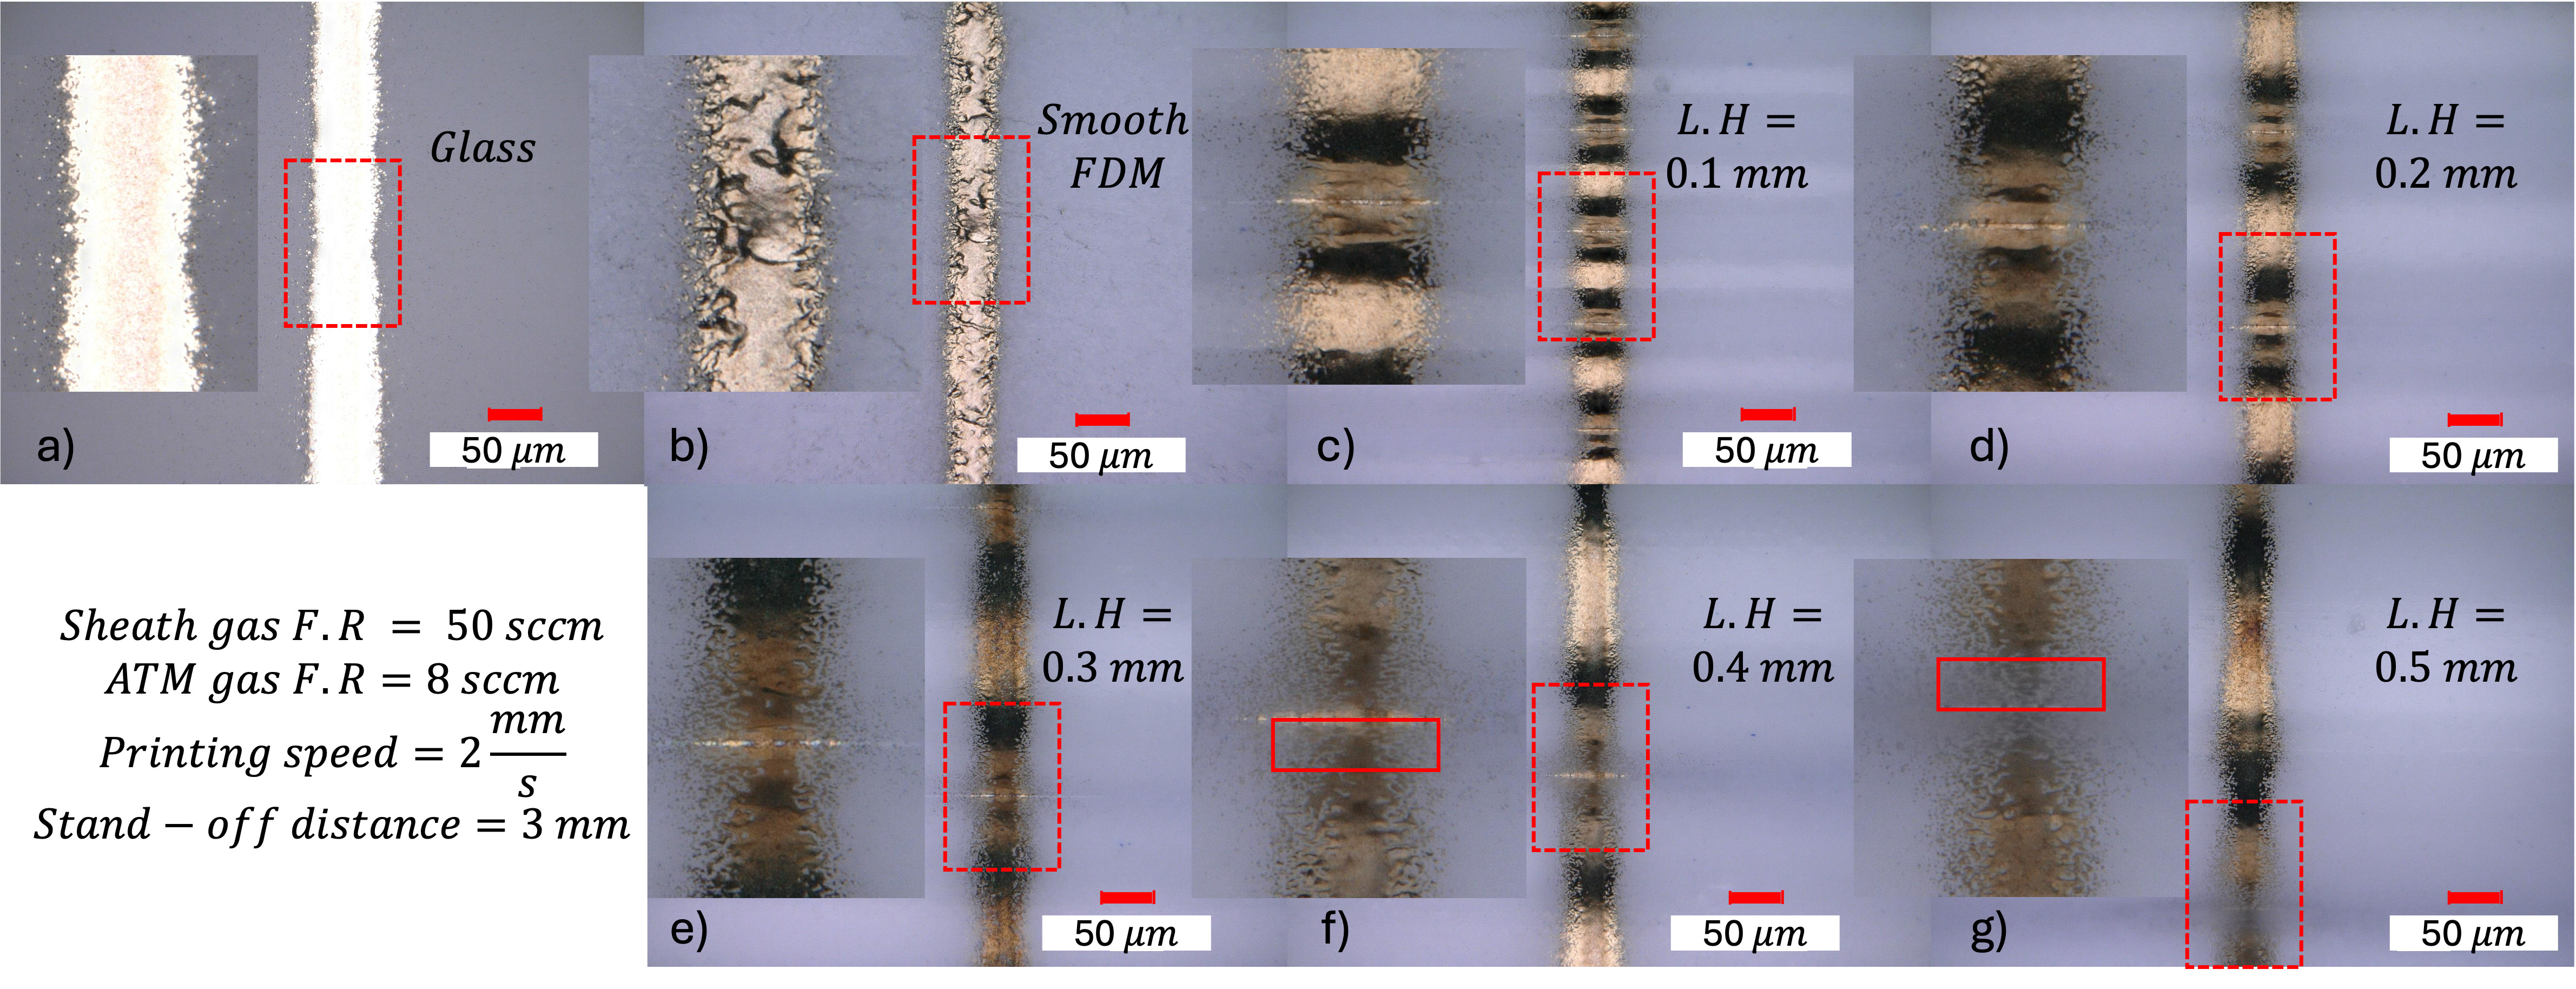
\includegraphics[width=1\linewidth]{figs/Picture1.jpg}
    \caption{Microscopy images of AJP-printed silver traces on glass, smooth FDM, and FDM substrates with varying layer heights.}
    \label{fig:result1}
\end{figure*}





\subsection{Part Design and Path Planning}
%%%%%%%%%%%%%%%%%%%%%%%%%%%%%%%%%%%%%%%%%%%%%%%%%%%%%%%%%%%
\subsubsection{FDM design}:
The PLA base plates exhibited external dimensions of \(80~\mathrm{mm}\times22~\mathrm{mm}\) and a thickness of \(0.8~\mathrm{mm}\). These substrates were printed in vertical orientation as shown in Figure \ref{fig:method}~(a), where the Z-axis of the printer was aligned with the width of the plate, and the thickness was achieved through the deposition of two adjacent rasters along the Y-axis. The layer height was identified as the principal parameter for controlling the surface roughness of the sidewalls, which subsequently served as the printing surface for the AJP process. For this investigation, layer heights varied from \(0.1~\mathrm{mm}\) to \(0.5~\mathrm{mm}\), with increments of \(0.1~\mathrm{mm}\). All other FDM printing parameters were maintained constant throughout the fabrication process, including printing speed (\(60~\mathrm{mm/s}\)), nozzle temperature (\(210~^{\circ}\mathrm{C}\)), and bed temperature (\(60~^{\circ}\mathrm{C}\)). The cooling duct was modified to direct airflow along the x-axis through thin slots, designed to provide adequate convective cooling during the printing of thin vertical walls at a reduced fan load. Crucially, this directional airflow minimized the risk of asymmetric cooling and subsequent structural deformation \cite{wang2007fdmcooling}.

Based on the surface roughness model, the sidewall surface profile is approximated as a parabolic curve \cite{li2019theoretical}, described by:

\begin{equation}
    f_p(x) = -2 \left[ \frac{t - 2\epsilon_y}{(t - \epsilon_x)^2} \right] x^2 + 2 \left[ \frac{t - 2\epsilon_y}{(t - \epsilon_x)} \right] x.
\end{equation}

where $t$ represents the layer thickness (layer hight) and $\theta$ is the stratification angle. The parameters $\epsilon_x$ and $\epsilon_y$ are defined as error coefficients which quantify the deviation of layer thickness along the X and Y directions respectively. They are modeled as independent random variables following normal distributions determined through experimental measurements. These coefficients integrate the influence of various error sources \cite{ahn2009representation}, such as geometric inaccuracies, process parameter variations, machine imperfections, and environmental factors into the surface profile model.

% added section
 


To create a baseline for comparison with a smooth surface, a group of substrates was fabricated in alternative printing orientation. These substrates were oriented such that their primary printing surface lay flat on the hotbed, with the Z-axis of the printer aligned with the substrate's thickness. The top surface of these FDM-printed PLA base plates was subsequently utilized for the AJP process. To further enhance surface uniformity and minimize roughness, additional ironed skin layer was applied to this top surface. This post-processing step involved repeatedly passing a heated nozzle over the printed top layer. The thermal energy from the nozzle softened the deposited material, and the flat nozzle tip effectively smoothed the surface by redistributing the polymer in an even way \cite{alzyod2023ironing}. This ironing process was executed at the exact height of model's top surface, with a reduced line spacing of $0.1~\mathrm{mm}$ and significantly low material extrusion rate ($14\%$ of the nominal flowrate) \cite{benno2024ironing} to precisely fill inter-line gaps and achieve a planar smooth surface.

\subsubsection{AJP pattern design}: 
To ensure repeatability of the results, three lines were printed on the FDM substrates for each test condition. The line traces were designed in AutoCAD, and the path files were generated using the VM Tools extension. The path files were kept strictly 2D to maintain a constant deposition head height during printing, allowing us to isolate and study how groove regions in the substrate affect material deposition. Figure~\ref{fig:method}~(b) illustrates the pattern design and the orientation of the printed lines relative to the substrate's roughness pattern. The lines were oriented perpendicular to the roughness features to create the most extreme condition for abrupt changes in surface height.

\begin{table}[]
\centering % Centers the table on the page
\caption{Connectivity outcomes for all test cases under different AJP process conditions.} % Added a caption
\label{tab:2} % The label should come AFTER the caption
\begin{tabular}{@{}lcccc@{}} % 'l' for labels, 'c' for centered data
\toprule
           % & \multicolumn{1}{c}{Test 1} & \multicolumn{1}{c}{Test 2} & \multicolumn{1}{c}{Test 3} & \multicolumn{1}{c}{Test 4} \\ \midrule
\textbf{Surface}      & \textbf{Test 1}                   & \textbf{Test 2}                    & \textbf{Test 3}                    & \textbf{Test 4} \\ \midrule
% Surface    & connection                & connection                & connection                & connection                \\ \midrule
$L.H=0.1$    & $\checkmark$              & $\checkmark$              & $\checkmark$              & $\checkmark$              \\
$L.H=0.2$    & $\checkmark$              & $\checkmark$              & $\checkmark$              & $\checkmark$              \\
$L.H=0.3$    & $\times$                  & $\times$                  & $\checkmark$              & $\checkmark$              \\
$L.H=0.4$    & $\times$                  & $\times$                  & $\times$                  & $\times$                  \\
$L.H=0.5$    & $\times$                  & $\times$                  & $\times$                  & $\times$                  \\
{\it Smooth FDM} & $\checkmark$              & $\checkmark$              & $\checkmark$              & $\checkmark$              \\
\textit{Glass}      & $\checkmark$              & $\checkmark$              & $\checkmark$              & $\checkmark$              \\ \bottomrule
\end{tabular}
\end{table}


\begin{figure}[h]
    \centering
    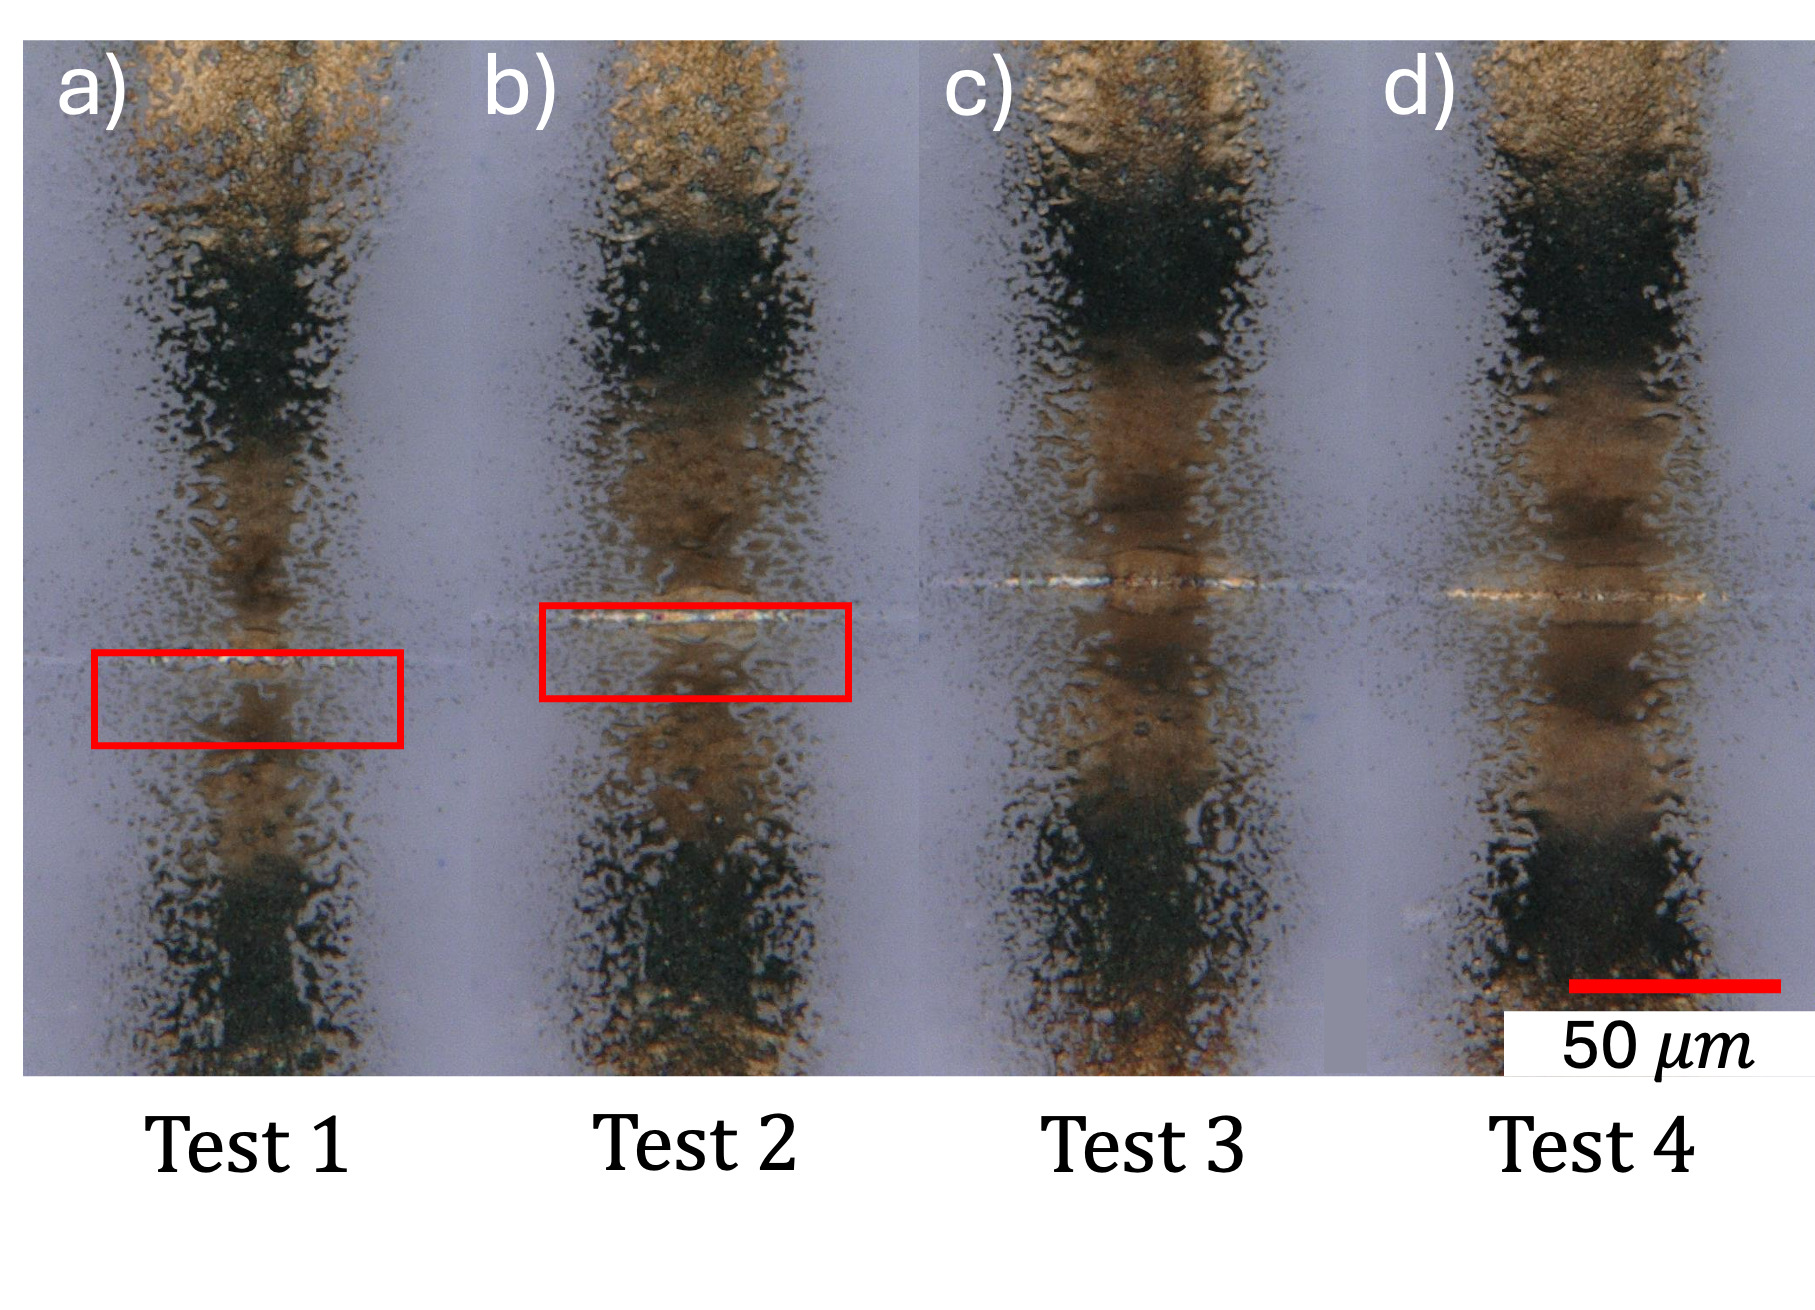
\includegraphics[width=1\linewidth]{figs/Picture222.jpg}
    \caption{High-resolution microscopy images of AJP lines printed on an FDM substrate with 0.3 mm layer height under four process conditions.}
    \label{fig:result2}
\end{figure}

\begin{figure}[h]
    \centering
    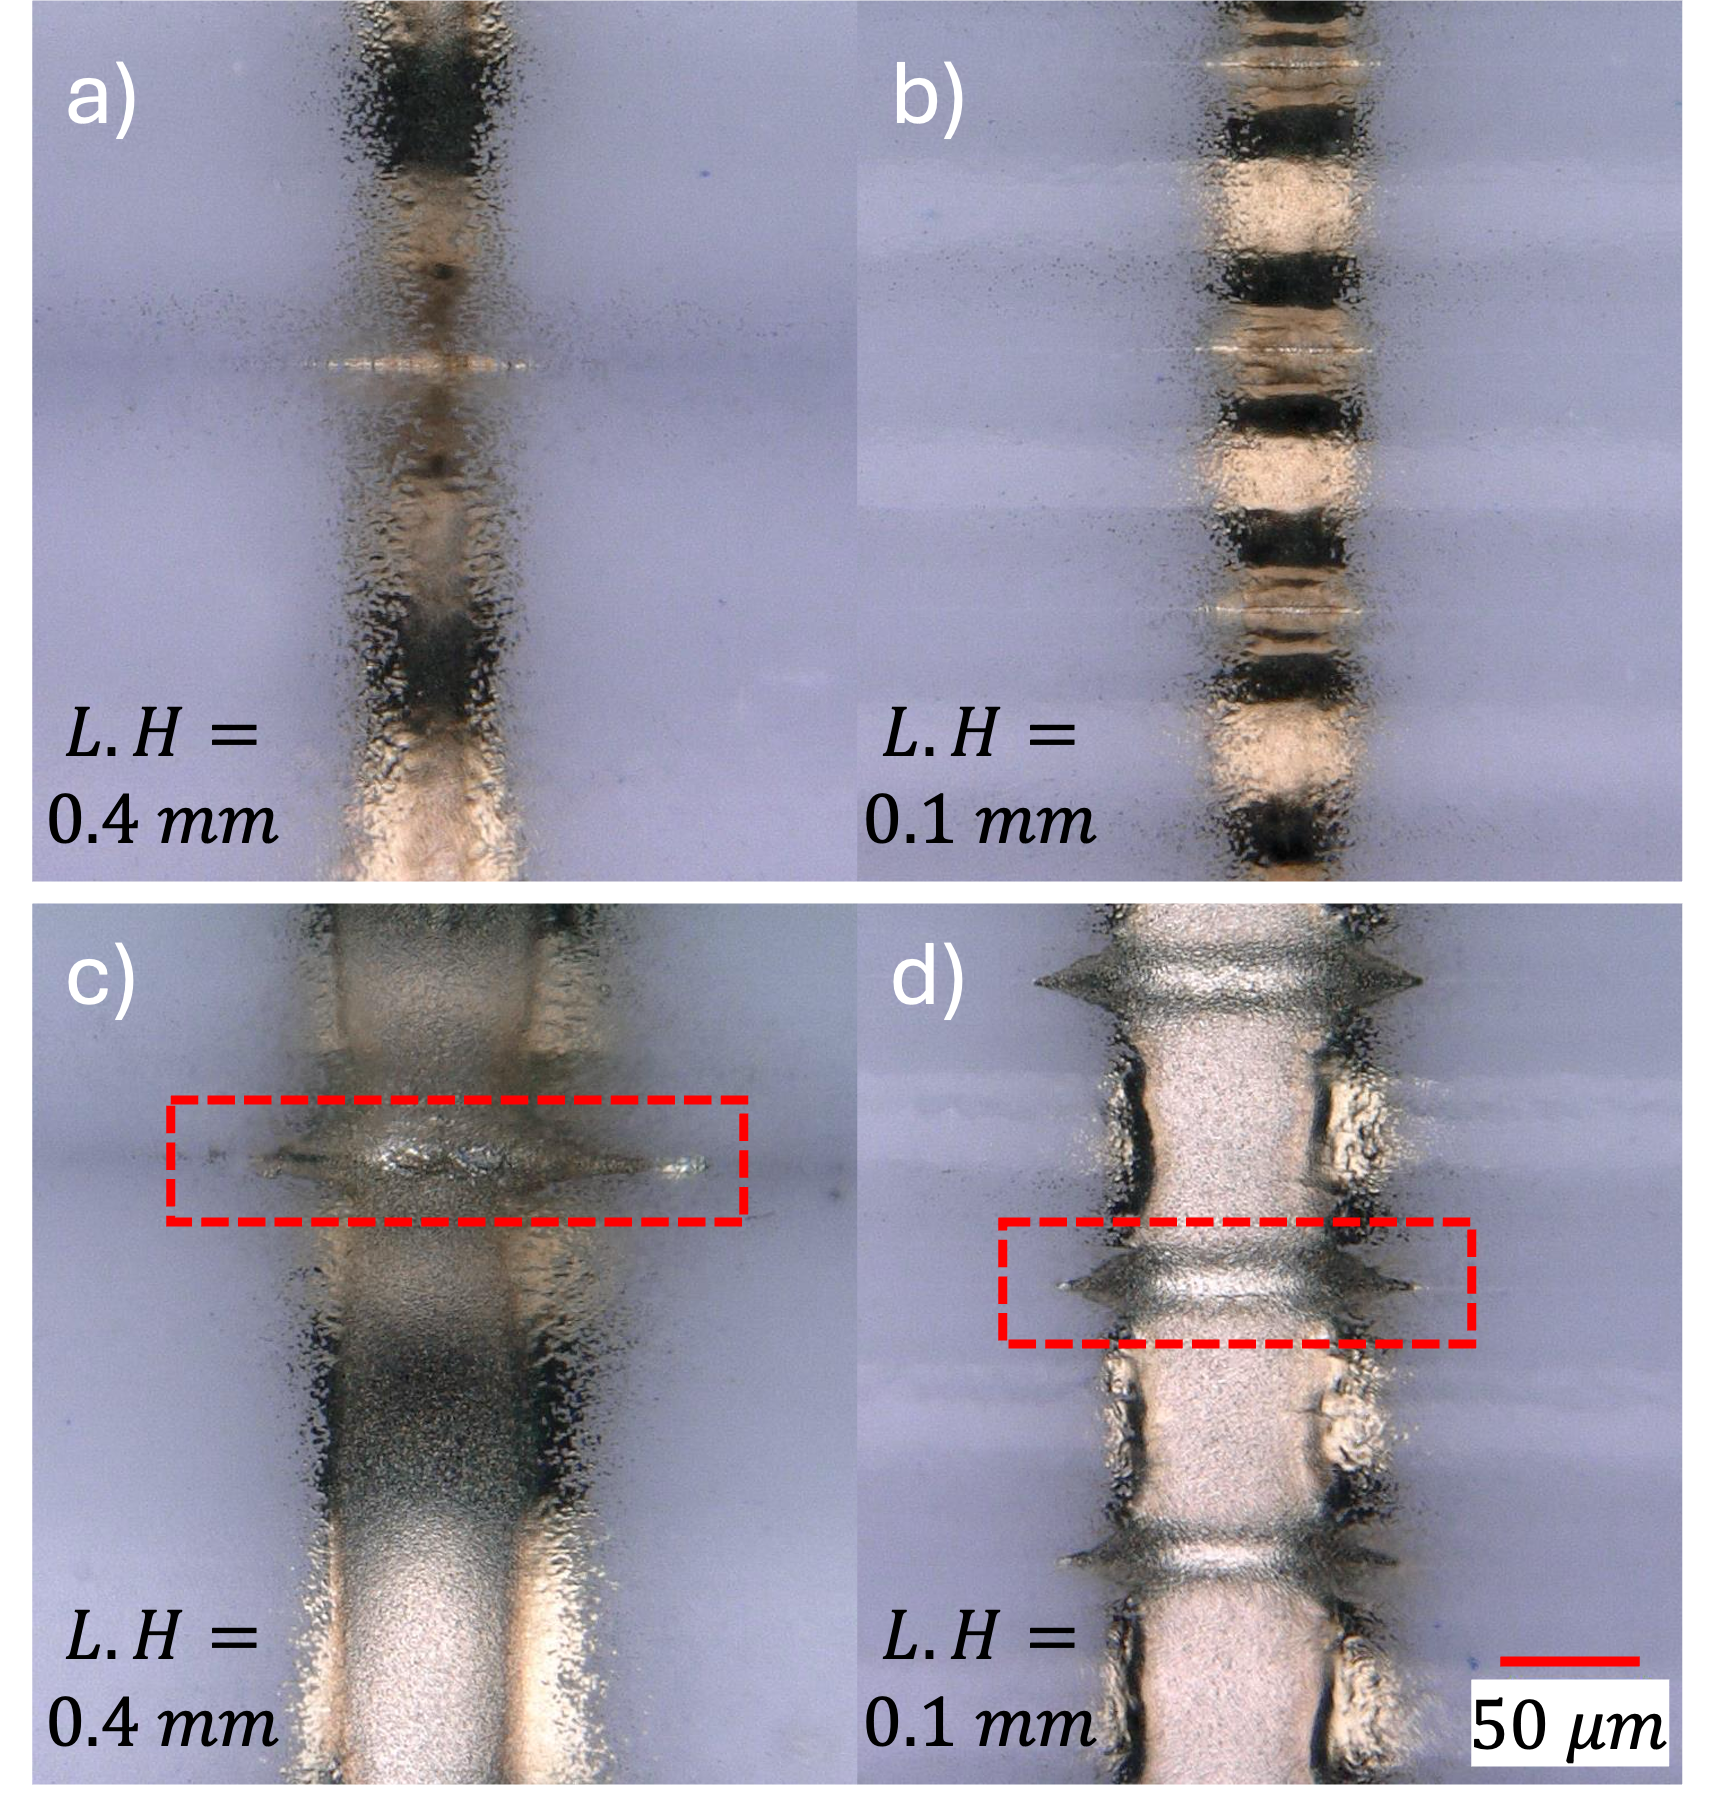
\includegraphics[width=1\linewidth]{figs/fig6.png}
    \caption{Optical microscopy images of AJP-printed lines on rough substrates under two deposition conditions: (a–b) baseline parameters (Test Condition 3, carrier gas flow rate \(8~\mathrm{sccm}\) and sheath gas flow rate \(50~\mathrm{sccm}\)) and (c–d) higher deposition rate (carrier gas flow rate \(20~\mathrm{sccm}\) and sheath gas flow rate \(40~\mathrm{sccm}\)) with constant print speed and stand-off distance, for L.H. = 0.1 mm and 0.4 mm. Higher deposition rate preserves continuity at L.H. = 0.4 mm but increases line width and material accumulation within surface grooves (red rectangles). All images are shown at identical magnification.}
    \label{fig:fig6}
\end{figure}

\begin{figure*}
    \centering
    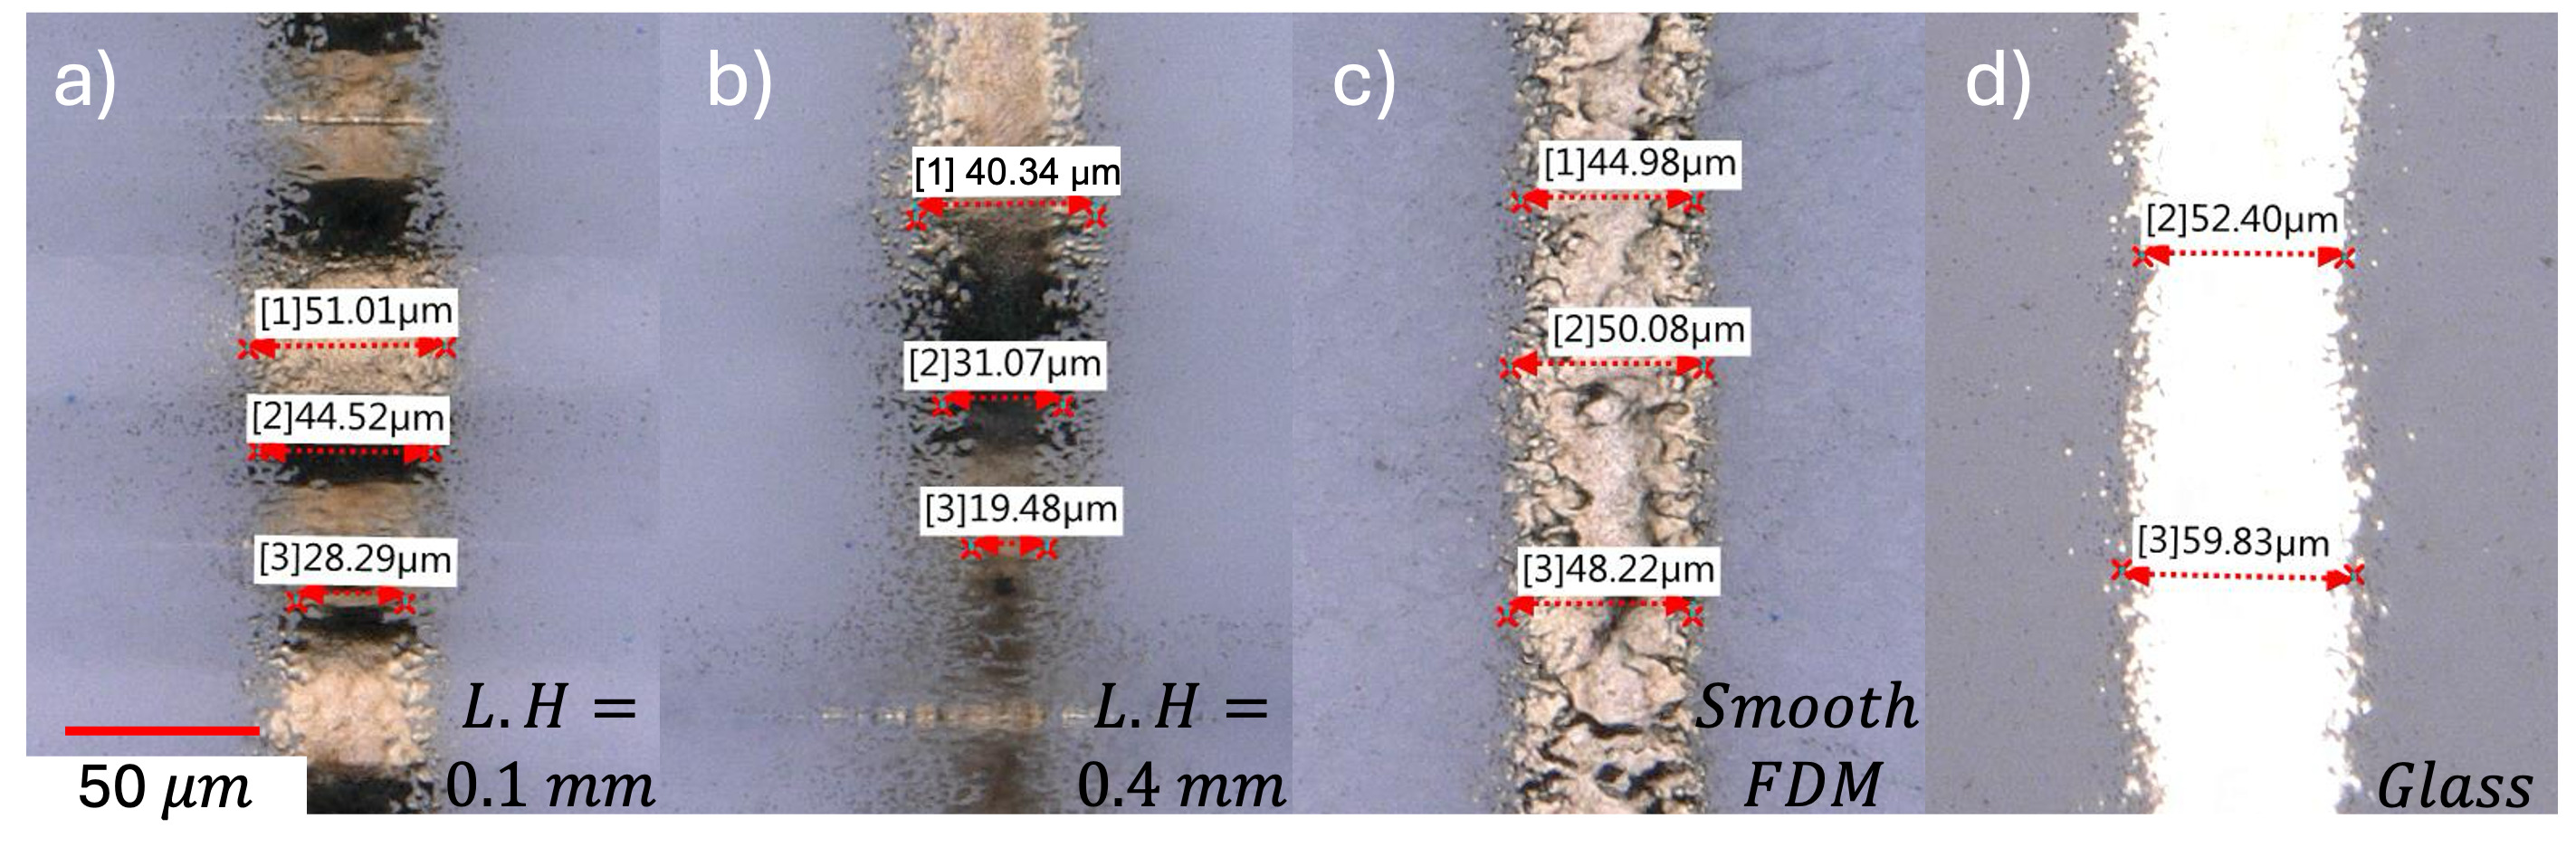
\includegraphics[width=1\linewidth]{figs/Picture3.jpg}
    \caption{Line width measurements for representative substrates with varying surface roughness.}
    \label{fig:result3}
\end{figure*}


\section{Results and Discussion}

This section presents the experimental results and line characterization used to evaluate material connectivity in AJP-printed silver traces on FDM substrates with varying layer heights. First, seven test samples printed under identical process parameters are examined to isolate the effect of layer height on deposition quality. Next, the overall evaluation of all test cases with respect to line connection is summarized. For one selected layer height, where line connectivity changes noticeably due to process variations, microscopic images obtained under different printing conditions are analyzed to assess how small parameter adjustments influence final line continuity. To provide additional quantitative insight, line width measurements are also reported for four representative substrates, including smooth FDM and glass as reference surfaces.

\subsection{Effect of Layer Height Under Fixed Process Parameters}

Figure \ref{fig:result1} shows microscopy images of the printed silver traces on a glass substrate, a smooth FDM surface, and five FDM surfaces with different layer heights (labeled accordingly). In the images of the rough substrates, the darker shaded regions correspond to groove valleys, while the brighter areas represent the crest of each printed layer. For each subfigure (a–g), a magnified region marked with a red dashed rectangle is included to highlight the groove area and enable clearer inspection of line continuity.

All samples in this experiment were printed under the same process parameters: sheath gas flow rate = 50 sccm, atomizer gas flow rate = 8 sccm, print speed = 2 mm/s, and a standoff distance of 3 mm. This allows the effect of layer height to be isolated as the primary variable.

Comparing Fig \ref{fig:result1}~(a) and (b), the silver traces printed on glass and on smooth FDM both show fully connected lines. However, the inherent surface roughness of the FDM substrate results in a visibly less uniform line surface compared to the glass reference. The roughness is further emphasized once the silver ink fills the micro-valleys, causing the printed line to highlight these surface variations.

The zoomed regions for the 0.1 mm, 0.2 mm, and 0.3 mm layer-height samples show continuous traces, although clear degradation in print quality is observed as layer height increases. At 0.3 mm, particle deposition becomes visibly less uniform, and the line morphology begins to show signs of thinning near the groove regions.

This trend continues for the 0.4 mm and 0.5 mm layer-height samples, where the enlarged views reveal distinct discontinuities in the groove valleys (highlighted with red rectangles). These disconnections confirm the significance of surface roughness in determining final line connectivity. As explained earlier, increasing layer height (t) increases groove depth. When the aerosol jet passes over a deeper groove at constant speed and deposition rate, the number of particles delivered per unit surface area becomes insufficient to fill the additional surface introduced by the roughness. Consequently, particle spacing increases, leading first to thinning of the trace and eventually to visible open gaps.

These results clearly demonstrate how progressively deeper grooves directly reduce material continuity. After establishing the influence of layer height alone, the next step is to investigate whether small adjustments in process parameters can compensate for these effects and improve the final electrical connection.




\subsection{Sensitivity of Line Connectivity to Printing Parameters}
Table~\ref{tab:2} presents the seven test cases printed under the four different conditions listed in Table~\ref{tab:1}. In this table, the check marks indicate lines with full continuity, while the "x" marks represent lines with gaps or disconnections. As observed, the glass substrate, the smooth FDM surface, and the layer heights of 0.1 mm and 0.2 mm consistently produce fully connected lines under all test conditions. In contrast, the layer heights of 0.4 mm and 0.5 mm always show disconnections in the groove regions.

The layer height of 0.3 mm demonstrates borderline behavior: it results in connected lines in Tests 3 and 4, but disconnected lines in Tests 1 and 2, where the print speed is higher. To examine this behavior more closely, Figure~\ref{fig:result2} shows high-resolution microscopy images of the printed lines on the 0.3 mm surface under all four process conditions. In the first two test cases, the red rectangles highlight the regions where the line becomes disconnected.

From these images, it is evident that the overall line quality improves progressively from Test 1 to Test 4. This supports the understanding that lower print speed increases the amount of particle deposition per unit area, resulting in better continuity and overall line morphology. Additionally, reducing the standoff distance (between Tests 1 and 2, and between Tests 3 and 4) decreases particle overspray and confines the aerosol plume more tightly, further enhancing particle-to-particle connectivity.

As shown in the figure, the surface with a 0.3 mm layer height lies at the threshold between connected and disconnected behavior. With only minor adjustments, either lowering the print speed or reducing the standoff distance, the line quality can improve significantly, without requiring any additional process modifications.


\subsection{\rev{Deposition Rate–Roughness Trade-Off in Line Continuity and Width Stability}}

\rev{To further examine whether surface roughness primarily affects printed lines at low deposition rates (i.e., low carrier gas flow) or whether roughness-induced defects also persist at higher deposition rates, additional experiments were conducted. Representative cases corresponding to layer heights (L.H.) of 0.1 mm and 0.4 mm were repeated under a new set of process parameters. Figure \ref{fig:fig6} presents optical microscopy images of the two surface conditions under two different processing settings. Figures~\ref{fig:fig6} (a) and (b) correspond to the same parameters as Test Condition 3. In Figures~\ref{fig:fig6} (c) and (d), the print speed and stand-off distance were kept constant, while the carrier gas and sheath gas flow rates were modified to increase the deposition rate.}

\rev{Under the revised condition, increasing the carrier gas flow increases the number of aerosol particles delivered to the substrate. As observed in the images, line continuity is preserved for the L.H. = 0.4 surface under the higher deposition rate, whereas the previous process condition resulted in discontinuity for the same surface (see Fig~\ref{fig:fig6}(a)). This indicates that increasing deposition rate can partially compensate for roughness-induced discontinuities.}

\rev{For both layer heights, an increase in carrier gas flow (i.e., deposition rate) also results in a noticeable increase in line width. The microscopy images are presented at identical magnification to enable direct visual comparison. Variations in line width between peak and groove regions remain visible in Figures~\ref{fig:fig6} (c) and (d), similar to the trends observed in Figures~\ref{fig:fig6} (a) and (b).}

\rev{However, a new phenomenon emerges under the higher deposition rate conditions. As highlighted by the red rectangles in Figures~\ref{fig:fig6} (c) and (d), there is a significant accumulation of material within the surface grooves. Because the deposited ink remains in a liquid state immediately after impact, capillary-driven flow and gravitational settling promote particle migration toward the bottom of the grooves. This results in localized ink enrichment, which subsequently spreads laterally along the groove direction, increasing the effective line width. This groove-driven accumulation increases line width variability and geometric inconsistency along the printed trace, which is undesirable for precision electronics applications. Furthermore, if the lateral migration of material becomes sufficiently severe, excessive spreading may cause unintended electrical connection with adjacent features in complex patterns, potentially leading to short-circuit defects.}

\rev{These results demonstrate that surface roughness not only influences high-resolution, low-deposition-rate printing, but also affects printing at higher deposition rates. Even when wider lines are produced under higher deposition conditions, roughness-induced flow redistribution and material accumulation can generate new classes of defects. Therefore, surface roughness must be explicitly considered during process parameter optimization for reliable AJP trace fabrication.}


\subsection{Quantitative Analysis of Line Width Variability}

Beyond line connectivity, the stability of line width serves as an additional indicator of print quality, as minimal width variation typically reflects more uniform particle deposition. To assess this effect, Figure~\ref{fig:result3} presents measured line widths for four representative cases:
\ref{fig:result3}(a) an FDM substrate with a 0.1 mm layer height, exhibiting surface roughness but maintaining good line connectivity;
\ref{fig:result3}(b) a 0.4 mm layer height, where the increased roughness leads to line discontinuities;
\ref{fig:result3}(c) smooth FDM; and
\ref{fig:result3}(d) glass, included as reference surfaces.

A clear contrast emerges when comparing cases \ref{fig:result3}(a) and \ref{fig:result3}(b)  with cases \ref{fig:result3}(c) and \ref{fig:result3}(d). Lines printed on smooth FDM and glass show the smallest variation in width, typically between 2–7 µm, demonstrating more consistent deposition. In contrast, the line printed on the 0.4 mm layer height substrate exhibits fluctuations as large as 20 µm. Notably, in case \ref{fig:result3}(b), the narrowest line width corresponds to the groove region where the line disconnect occurs, indicating insufficient particle accumulation to bridge the deeper valleys. A similar, though less severe, reduction in line width is observed for case \ref{fig:result3}(a), where the groove width remains smaller than the peak regions. This suggests that while the line remains connected at a 0.1 mm layer height, it is more vulnerable to cracking or disconnection if any deformation occurs in the substrate.

When comparing smooth FDM and glass, both show low variability, but the average line width on glass is approximately 10 µm larger under identical process conditions. This highlights the effect of surface smoothness: the ultra-smooth glass surface facilitates more lateral spreading and easier particle mobility, whereas the FDM surface, even when smoothed, retains micro-scale texture that slightly restricts deposition.

Overall, the results clearly demonstrate that surface roughness significantly influences particle deposition per unit area in high-resolution AJP printing. As groove depth increases, insufficient particle delivery leads to reduced local deposition density, trace thinning, discontinuities, and line-width variations that exceed the typical range observed in AJP. \rev{In contrast, at higher deposition rates (corresponding to lower-resolution, wider lines), surface roughness promotes localized particle accumulation within groove regions, leading to undesirable line-width expansion.} While these findings provide important insight into an existing knowledge gap for hybrid printed electronics, particularly when AJP traces are deposited on additively manufactured substrates with defined roughness profiles, further comprehensive studies are needed to establish quantitative relationships and develop predictive models. Although the simple process variations explored here showed partial effectiveness in improving line continuity, more systematic investigations are required to fully understand the underlying mechanisms and to identify robust optimization strategies.

%%%%%%%%%%%%%%%%%%%%%%%%%%%%%%%%%%%%%%%%%%%%%%%%%%%%%%%%%%%
\section{Conclusion}
This study examined the influence of substrate surface roughness, specifically, the layer-height–induced roughness of FDM-printed parts, on the quality and continuity of aerosol jet printed conductive traces. Glass and smooth FDM substrates were used as baseline references, while FDM surfaces with layer heights ranging from 0.1 mm to 0.5 mm were evaluated to represent systematically increasing roughness amplitudes.

\rev{Under low deposition rate conditions,} the results demonstrate that substrate roughness has a significant effect on particle deposition during AJP. As layer height increased, the depth of surface grooves introduced additional surface area that could not be sufficiently covered under fixed deposition conditions. This led to progressively reduced local deposition density, thinning of the printed trace, and ultimately loss of line connectivity. The 0.3 mm layer height emerged as a threshold case: under standard parameters, this surface exhibited borderline behavior, with continuity failing in some conditions but preserved in others.

To further examine process robustness \rev{while maintaining the baseline process parameters}, four modified printing conditions were tested by adjusting standoff distance and print speed. These simple parameter variations were able to partially compensate for roughness-related deposition deficits, illustrating that, for borderline surfaces, even modest increases in particle delivery per unit area can restore connectivity. However, highly rough surfaces (0.4 mm and 0.5 mm layer height) consistently resulted in disconnected traces, regardless of parameter adjustments.

\rev{The results at higher deposition rates indicate that the influence of surface roughness is not limited to high-resolution conditions; rather, it introduces a different class of defects while maintaining line continuity. Increased particle delivery promotes material accumulation and redistribution within surface grooves, resulting in line-width expansion. In densely patterned layouts, this excessive lateral spreading may lead to unintended electrical bridging. These findings reveal a trade-off between deposition rate and geometric stability: higher deposition rates improve connectivity but increase the risk of width variability and potential short-circuit formation, whereas lower deposition rates increase the likelihood of discontinuities. This behavior underscores the need for systematic, multi-parameter optimization strategies.} 

Quantitative line-width analysis reinforced these findings. Compared to glass and smooth FDM, rough surfaces exhibited significantly larger variations in line width, particularly within groove valleys where deposition was insufficient. These variations highlight both the sensitivity of high-resolution AJP to micro-scale topography and the potential risk for crack formation or electrical failure when printing on additively manufactured substrates.

Overall, the results emphasize the importance of jointly considering the characteristics of multiple additive manufacturing processes when integrating them into hybrid workflows. A parameter change in one process, such as the selected layer height in FDM, can directly influence the printability and electrical performance of subsequent AJP layers.

Future work will include expanding the process window with additional printing parameters \rev{and exploring a broader range of process variables}, integrating other AM technologies such as stereolithography (SLA), and employing CFD-based simulations to model gas and particle behavior over rough surfaces. \rev{The findings may further be integrated with classification-based predictive models to enable pre-print process planning and defect anticipation.} These efforts will support a deeper understanding of the underlying physics and will inform reliable optimization strategies for printing high-quality electronics on complex geometries.

Collectively, this study highlights the need for continued investigation into hybrid additive manufacturing, particularly the interaction between structural AM processes and functional AJP deposition. The insights provided here contribute toward enabling reliable, high-quality printed electronics on diverse materials and surfaces, whether embedded within or deposited onto additively manufactured components.

\section*{Acknowledgment}
This publication is supported in part by the Joint Research Project between the University Academic Alliance in Taiwan and the University of Illinois System.
\bibliographystyle{asmejour}  %% .bst file following ASME journal format. Do not change.
\bibliography{asmeconf-sample}%% bibliography file


 

\end{document}
